%-------------------------------------------------------------------------------
%                            BAB III
%               		METODOLOGI PENELITIAN
%-------------------------------------------------------------------------------

\chapter{METODOLOGI PENELITIAN}

\section{Tempat dan Waktu Penelitian}
\setlength\parindent{30pt} Penelitian ini dilakukan di Laboratorium Pemrograman dan Database (PDB), Jurusan Informatika, Fakultas Matematika dan Ilmu Pengetahuan Alam, Universitas Syiah Kuala, Darussalam, Banda Aceh. Estimasi waktu yang dibutuhkan untuk penelitian ini terhitung dari bulan Februari 2018 sampai dengan bulan Agustus 2018.

\section{Alat dan Bahan}
Alat yang digunakan pada penelitian ini adalah sebagai berikut :

\begin{enumerate}[a.]
\item Perangkat Keras (\textit{Hardware})
	\begin{itemize}
		\item 1 unit Laptop HP Intel(R) Core(TM) i3
		\item RAM 6 GB DDR3
		\item Harddisk 500 GB
		\item 1 unit Android Xiaomi Redmi 4A RAM 2GB
	\end{itemize}

\item Perangkat Lunak (\textit{Software})
	\begin{itemize}
		\item Sistem Operasi Windows 10
		\item XAMPP versi 5.6.30
		\item Apache Tomcat 7.0.56
		\item Sublime Text versi 3
		\item Android Studio versi 3.0.1
		\item IntelliJ IDEA 2018.1.1

	\end{itemize}
\end{enumerate}

\section{Metode Kerja}
Metode kerja yang akan dilakukan pada penelitian ini dapat dilihat pada gambar 3.1. Berikut penjelasan alur metode kerja yang akan dilakukan.
	\begin{figure}[H]
		\centering
		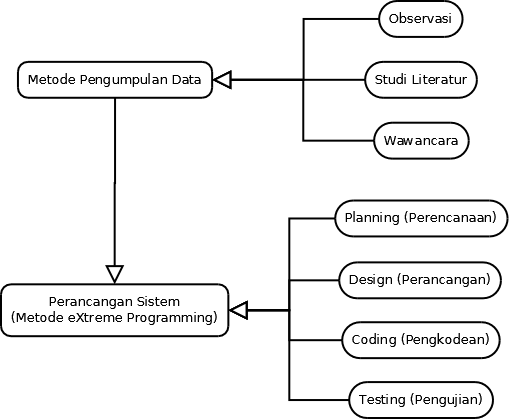
\includegraphics[scale=0.5]{gambar/alur}
		\caption{Alur diagram metode kerja}
		\label{alur}
	\end{figure}

\subsection{Metode Pengumpulan Data}
Metode pengumpulan data pada penelitian ini ada tiga yaitu:
\begin{enumerate}[a.]
	\item Observasi, dilakukan dengan melihat langsung media promosi yang dilakukan oleh pemilik kos, yaitu pamplet, brosur, \textit{broadcast} aplikasi \textit{chatting}. Melihat informasi apa saja yang tertera pada media promosi tersebut.
	\item Studi literatur, tahap ini adalah tahap pengumpulan data dengan cara membaca dan mempelajari literatur yang berhubungan dengan penelitian ini seperti Android, \textit{web service}, pengembangan aplikasi, kode QR, pengujian aplikasi, analisa kebutuhan, \textit{problem frames}, OCL dan lain-lain.
	\item Wawancara, metode ini dilakukan dengan cara mewawancarai \textit{user} yaitu pencari kos dan pemilik kos yang berhubungan dengan mencari dan menyediakan kos. Hal ini dilakukan untuk mendapatkan kebutuhan terhadap aplikasi yang akan dibangun. 
\end{enumerate}

\subsection{Perancangan Sistem}
Perancangan aplikasi pencarian kos-kosan ini adalah dengan menggunakan metode \textit{Agile Software Development} jenis \textit{eXtreme Programming} (XP). Tahapan dari \textit{eXtreme Programming} (XP) adalah sebagai berikut:

\begin{enumerate}[a.]
\item \textit{Planning} (Perencanaan)

Tahap perencanaan ini dimulai dengan mengumpulkan kebutuhan-kebutuhan untuk aplikasi yang akan dikembangkan dalam bentuk cerita (\textit{user stories}). \textit{User stories} menggambarkan keluaran yang diperlukan, fitur-fitur dan fungsionalitas-fungsionalitas aplikasi.  Untuk mendapatkan \textit{user stories}, maka akan dilakukan wawancara kepada \textit{user} atau orang yang akan menggunakan aplikasi ini. \textit{User} yang akan diwawancara adalah pemilik kos dan mahasiswa sebagai pencari kos atau anak kos. Pencarian \textit{user} dilakukan dengan cara mendatangi beberapa kos yang tersebar di daerah Banda Aceh. 
	
Langkah selanjutnya adalah menganalisa kebutuhan yaitu mendeskripsikan masalah dengan menjabarkan \textit{requirement}, \textit{domain knowledge}, dan mengidentifikasikan domain yang relevan dan \textit{share phenomena}. Setelah masalah sudah terkumpul, kemudian masalah tersebut akan dibagi ke dalam sub masalah dengan cara mengidentifikasikan kebutuhan-kebutuhan yang saling berkaitan. Sub masalah ini akan dicocokkan ke dalam \textit{problem frames} yang dinyatakan dalam \textit{frame diagrams}. Setelah mendapatkan \textit{frame diagrams}, akan dianalisa lagi menggunakan UML diagram kelas dan notasi spesifikasi formal OCL.
	
\item \textit{Design} (Perancangan)
	
Tahap perancangan akan dimulai dari merancang basis data dan \textit{interface} aplikasi. Basis data digunakan untuk menyimpan data kos-kosan yang di\textit{input} oleh pemilik kos. Aplikasi yang dibangun dibagi menjadi 2 bagian, yaitu web untuk pemilik kos dan Android untuk pencari kos. Berikut adalah \textit{mockup} aplikasi yang akan dibuat untuk pencari kos:
	
	\begin{figure}[H]
		\centering
		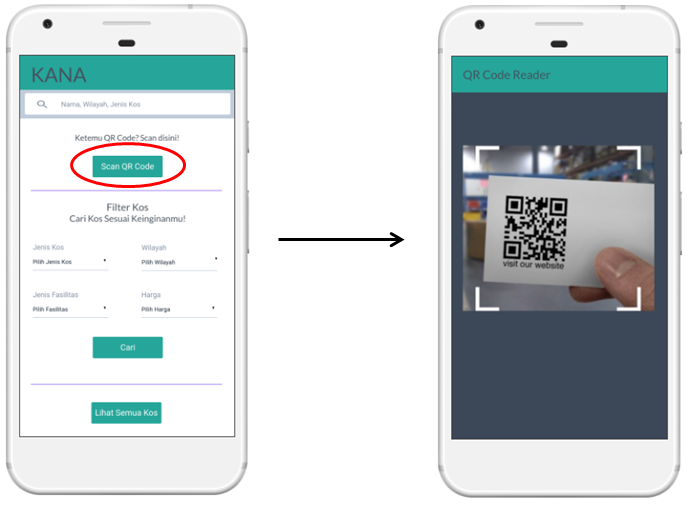
\includegraphics[width=\linewidth]{gambar/and1}
		\caption{Tampilan utama aplikasi Android (kiri) dan tampilan QR Code Reader jika menekan tombol Scan QR Code pada tampilan utama (kanan)}
		\label{android1}
	\end{figure}
	
Gambar \ref{android1} adalah ketika menekan tombol \textit{Scan QR Code}, akan menampilkan kamera yang digunakan untuk memindai kode QR. Jika kode QR dapat dibaca, maka akan menampilkan informasi mengenai kos yang memiliki kode QR tersebut.
	
	\begin{figure}[H]
		\centering
		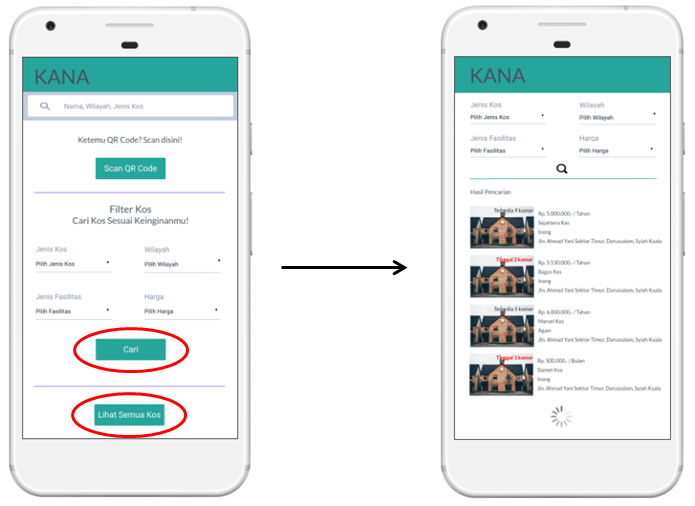
\includegraphics[width=\linewidth]{gambar/and2}
		\caption{Tampilan halaman jika menekan tombol Cari dan Lihat Semua Kos}
		\label{android2}
	\end{figure}
	
Gambar \ref{android2} adalah tombol Lihat Semua Kos yang akan menghasilkan halaman seluruh daftar kos-kosan yang ada dalam \textit{database}, tetapi tombol Cari akan menghasilkan daftar kos sesuai \textit{input} dari pengguna berdasarkan jenis, wilayah, fasilitas dan harga kos.
	
	\begin{figure}[H]
		\centering
		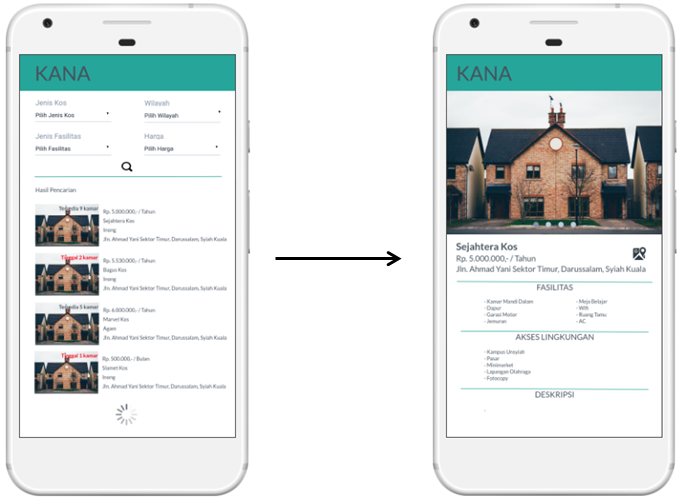
\includegraphics[width=\linewidth]{gambar/and3}
		\caption{Tampilan halaman jika menekan salah satu kos yang dicari}
		\label{android3}
	\end{figure}
	
Gambar \ref{android3} adalah halama dimana jika salah satu kos diklik, maka akan menampilkan halaman berupa informasi mengenai kos tersebut. 

Sedangkan \textit{mockup} aplikasi web untuk pemilik kos adalah sebagai berikut:
	
	\begin{figure}[H]
		\centering
		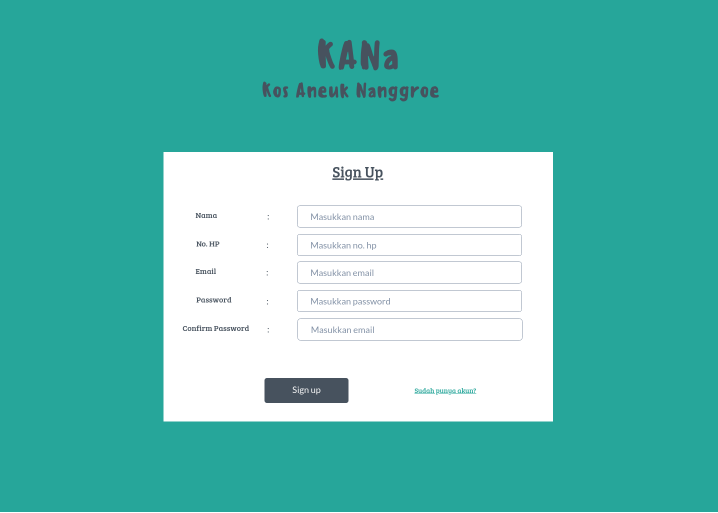
\includegraphics[scale=0.5]{gambar/web2}
		\caption{Tampilan halaman daftar akun kos}
		\label{webb2}
	\end{figure}
	
Gambar \ref{webb2} adalah halaman daftar bagi pemilik kos-kosan yang ingin mempromosikan kos miliknya. Jika menekan 'Sudah punya akun?', maka akan muncul halaman seperti pada gambar \ref{webb1}.
	
	\begin{figure}[H]
		\centering
		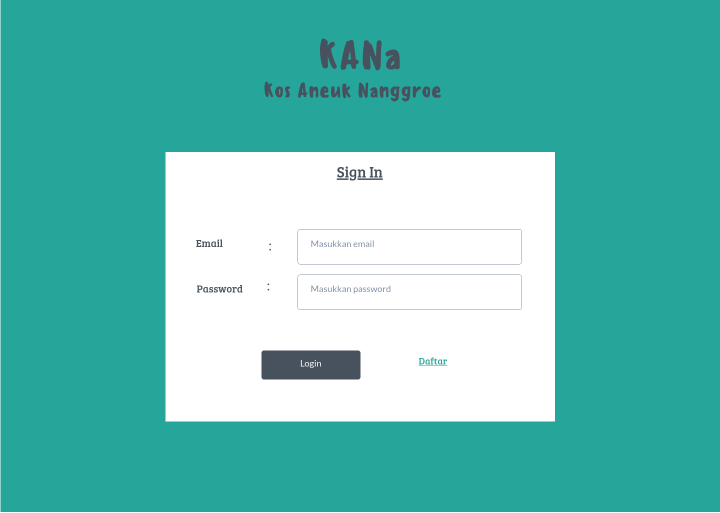
\includegraphics[scale=0.5]{gambar/web1}
		\caption{Tampilan halaman \textit{login} akun kos}
		\label{webb1}
	\end{figure}
	
Halaman \textit{login} pemilik kos. Setelah klik tombol \textit{Login}, akan menampilkan halaman seperti pada gambar \ref{webb3}.
	
	\begin{figure}[H]
		\centering
		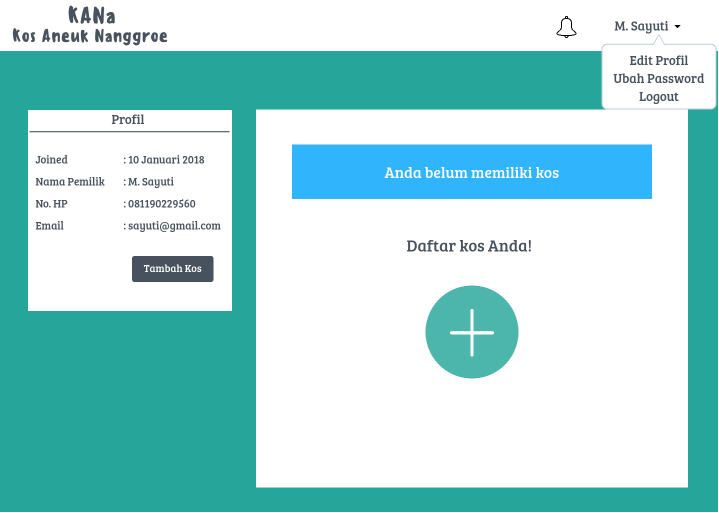
\includegraphics[scale=0.5]{gambar/web3}
		\caption{Tampilan halaman profil akun kos}
		\label{webb3}
	\end{figure}
	
Halaman profil ini akan menampilkan informasi pemilik kos yang terletak di sebelah kiri dan di sebelah kanan akan ditampilkan kos-kosan yang didaftarkan oleh pemilik kos. 
	
	\begin{figure}[H]
		\centering
		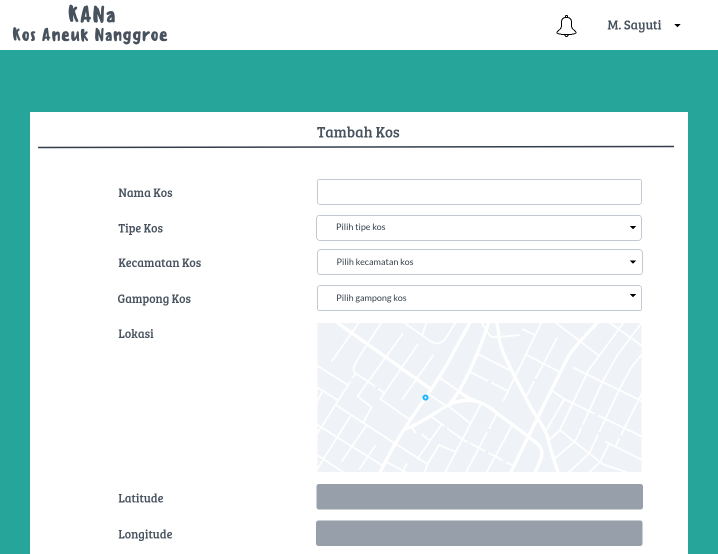
\includegraphics[scale=0.5]{gambar/web4}
		\caption{Tampilan halaman tambah kos}
		\label{webb4}
	\end{figure}
	
	\begin{figure}[H]
		\centering
		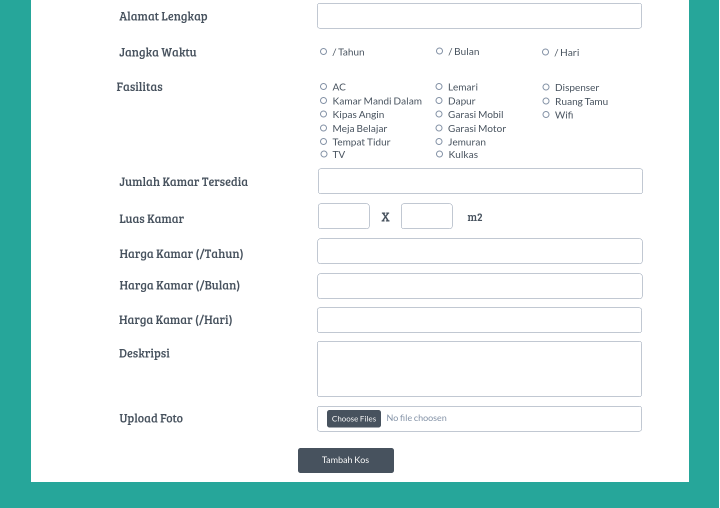
\includegraphics[scale=0.5]{gambar/web4a}
		\caption{Tampilan halaman tambah kos}
		\label{web4a}
	\end{figure}
	
Gambar \ref{webb4} dan \ref{web4a} adalah halaman untuk menambahkan data kosan. Tombol Daftar Kos untuk menyimpan data kos yang dimilikinya. Pemilik kos harus mengisi informasi-informasi yang telah disediakan. Setelah menyimpan data kos, maka akan muncul halaman awal dengan kos yang sudah berhasil di-\textit{input}.
	
	\begin{figure}[H]
		\centering
		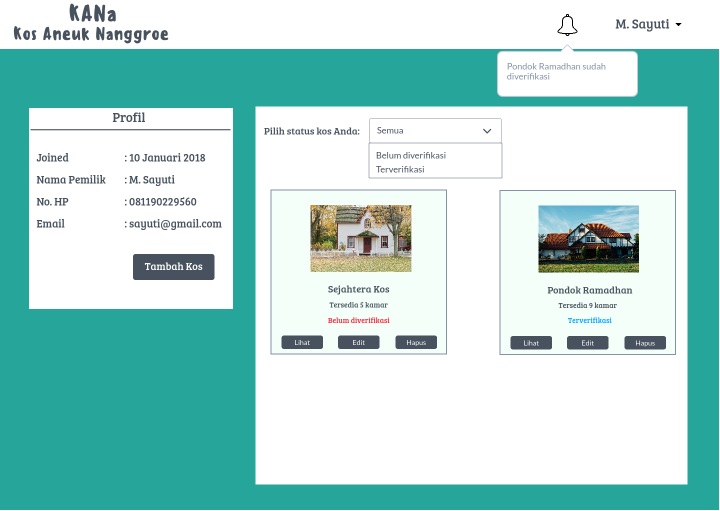
\includegraphics[scale=0.5]{gambar/web5}
		\caption{Tampilan halaman profil akun kos yang sudah ada kos-kosan}
		\label{webb5}
	\end{figure}
	
Pada halaman seperti gambar \ref{webb5}, pemilik kos dapat melihat kos yang sudah diverifikasi atau belum bahkan semua kos yang di-\textit{input}. Data yang sudah di-\textit{input} dapat dilihat, diedit dan dihapus. Untuk tombol Lihat dan Edit, akan menuju halaman seperti gambar \ref{webb4} dan gambar \ref{web4a}.
	
	\begin{figure}[H]
		\centering
		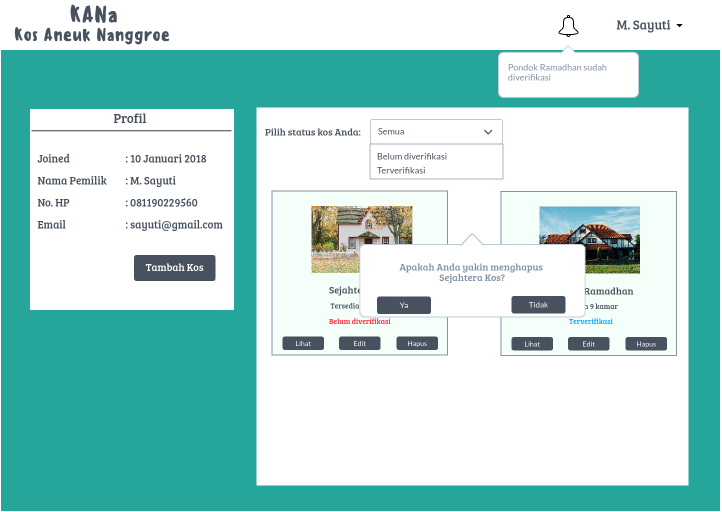
\includegraphics[scale=0.5]{gambar/web7}
		\caption{Tampilan halaman jika menekan tombol Hapus pada salah satu kos}
		\label{webb7}
	\end{figure}
	
	\begin{figure}[H]
		\centering
		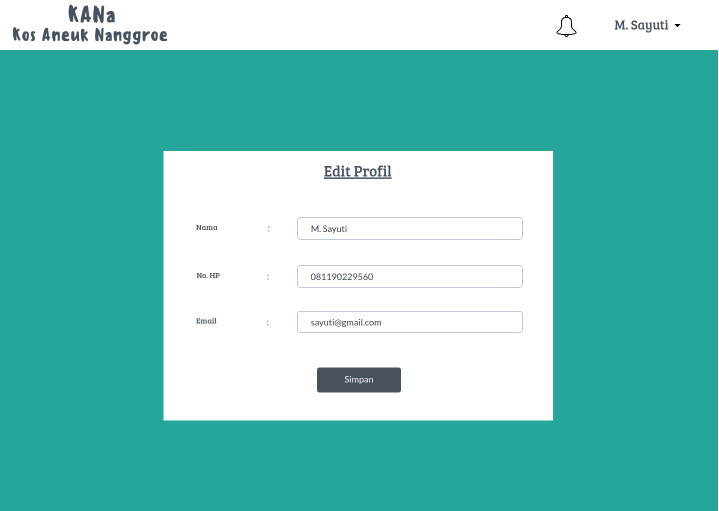
\includegraphics[scale=0.5]{gambar/web8}
		\caption{Tampilan halaman edit profil}
		\label{webb8}
	\end{figure}
	
	\begin{figure}[H]
		\centering
		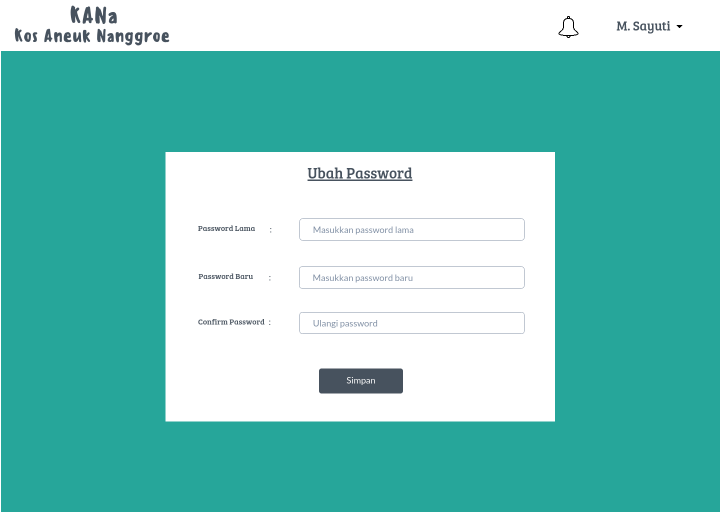
\includegraphics[scale=0.5]{gambar/web6}
		\caption{Tampilan halaman ubah password}
		\label{webb6}
	\end{figure}

	Pemilik kos juga dapat menghapus kos, edit profil dan mengubah password seperti pada gambar \ref{webb7}, \ref{webb8} dan \ref{webb6}.
	
	\item \textit{Coding} (Pengkodean)
	
Selanjutnya akan dilakukan penulisan program, pada penelitian ini menggunakan dua aplikasi yaitu web dan Android dan menggunakan \textit{web service} sebagai penghubung antara \textit{database }dan aplikasi Android. Pembuatan aplikasi web menggunakan \textit{framework} Laravel dan bahasa pemrograman PHP dan \textit{database} yang digunakan MySql. Untuk Android menggunakan bahasa pemrograman Java. Sedangkan \textit{web service} menggunakan RESTful API dengan \textit{framework} Jersey. Penulisan program ini akan membutuhkan PC untuk membuat aplikasi web dan menjalankan aplikasi Android Studio untuk membuat aplikasi \textit{mobile} serta \textit{smartphone} yang digunakan sebagai emulator Android Studio. 
	
	\item \textit{Testing} (Pengujian)
	
Pengujian yang dilakukan adalah pengujian \textit{usability} dengan metode \textit{System Usability Scale} (SUS). Pengujian ini dilakukan oleh pengguna akhir dari aplikasi yang akan dibangun. Hal ini bertujuan untuk mengetahui tingkat penerimaan pengguna, apakah aplikasi ini dapat diterima oleh pengguna atau tidak. Pengujian ini dilakukan kepada dua kelompok pengguna, yaitu pemilik kos dan pencari kos. Metode SUS dapat digunakan untuk mengukur kegunaan (\textit{usability}) dari suatu sistem dengan sampel yang kecil yaitu 2 pengguna \citep{brook1996}. Namun pada penelitian ini sampel yang digunakan adalah 30 pengguna per kelompok pengguna agar mendapatkan data yang lebih akurat.
\end{enumerate}


% Baris ini digunakan untuk membantu dalam melakukan sitasi
% Karena diapit dengan comment, maka baris ini akan diabaikan
% oleh compiler LaTeX.
\begin{comment}
\bibliography{daftar-pustaka}
\end{comment}
